The final histogram strategy is the histogram by sort, and is unlike the histogram by privatization very different from the naive strategy. The idea behind the histogram by sort is to first sort the input array, and then calculates the histogram based number of element within the given bin widths. The histogram by sort eliminates the thread contention which was the limiting factor in the naive and privatization strategies, but may introduce a lot of overhead caused by the sort algorithm. An visual example of the histogram by sort is seen in \cref{fig:hist_sort}. 

\begin{figure}[ht]
	\centering
	\fbox{
		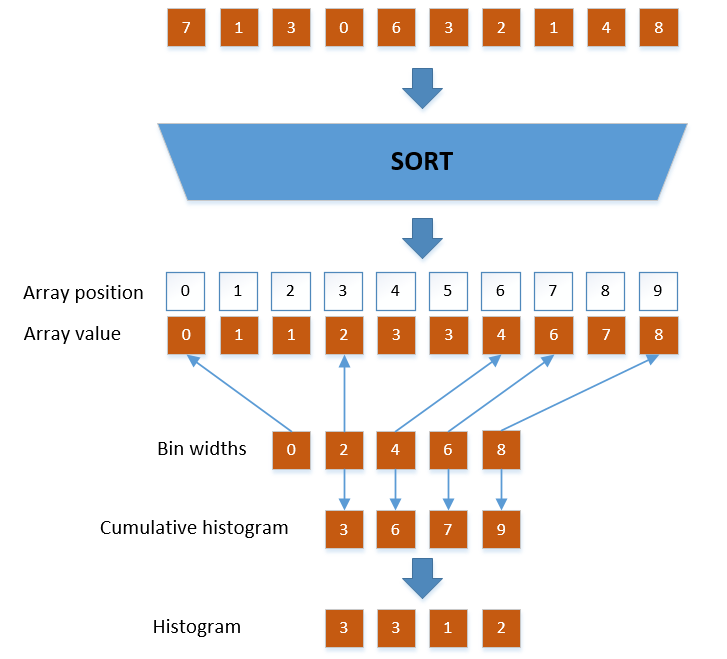
\includegraphics[width=0.5\textwidth]{figs/algorithm/hist_sort.png}}
	\caption{Histogram by sort}
	\label{fig:hist_sort}
\end{figure} 

Firstly, the input array is sorted using a parallel sorting algorithm, like the ones presented in \cref{sec:al_sort}. After the sorting the bin widths, predefined to the histogram function call, are used to find the upper bounds of array positions. The upper bound is found by writing the highest array position, of a specific bin width value to a new array, as seen in \cref{fig:hist_sort}. This upper bound array is the cumulative histogram, and the final histogram is then found by subtracting the left neighbour element from each element in the array. 
The histogram by sort has a high overhead because of the sorting, but may be better than the histogram by privatization, when the number of input element is high, the number of bins is high or when the input data is not uniformly distributed. In all of those cases the histogram by privatization will be limited by the serialization cause by the atomic operations. These are also the conclusions in the histogram study by \cite{MilicHistogram} and a final note is that parallel histogram strategies are highly application specific.